% !TEX root = tracking.tex
\section{Introduction}
 Currently there is a great interest both in research and industry to find methods of fast path planning for autonomous quadrotors and other vehicles. These vehicles must be able to plan and execute a dynamic trajectory in real-time without violating safety constraints. This is a very difficult challenge: the need for fast planning is generally at odds with the need for maintaining safety and robustness. In order to achieve real-time planning for any environment with static obstacles, researchers typically must use highly simplified model dynamics or kinematics, resulting in a tracking error between the planned path and the true high-dimensional system. This concept is illustrated in Figure \ref{fig:chasing}, where the path was planned using a simplified model (player 1), but the real vehicle (player 2) cannot follow this path exactly. In addition, most current planners do not consider the effect of external disturbance (e.g. wind) on the resulting tracking error. This tracking error due to the simplified dynamics and lack of disturbances can lead to unsafe situations in which the planned path may be safe, but the actual vehicle trajectory crashes into an obstacle or other unsafe region.

We propose a modular tool that will provide precomputed look-up tables to easily find online the maximum possible tracking error bound, as well as the optimal control for the vehicle to minimize this tracking error. We compute these tables by using Hamilton Jacobi reachability analysis to analyze a capture-avoid game in relative coordinates between the (potentially simplified) model used for fast planning and the (typically more sophisticated) model used to track the planner. Additional external disturbances can be included in this analysis. The result is a mapping that takes as an input the current relative state between the planning model and the tracking model, and outputs the optimal control to follow the planner along with the largest possible tracking error bound. This error bound captures all deviations due to nonlinearities and disturbance in the tracking system, and can be thought of as a "safety bubble" around the planning model (i.e. the path planner). We can prove that \textcolor{red}{statement of proof}. It is important to note that this precomputation is \textit{independent} of the path planned in real-time; what matters is the relative state between the systems, not the absolute state of the path. 

\begin{figure}
	\centering
	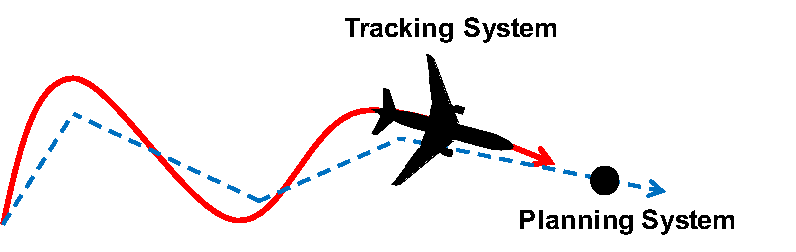
\includegraphics[width=0.47\textwidth]{fig/chasing}
	\caption{\textcolor{red}{filler image about quadrotors chasing each other}}
	\label{fig:chasing}
\end{figure}

This tool is designed to be modular and able to use in conjunction with sundry fast path and trajectory planners to add robustness and safety guarantees. In the online computation, the obstacles are first padded by the tracking error bound. These augmented obstacles are used by the planner to decide the next desired state using the planning model. The vehicle will then find the relative state between itself and this desired state. This relative state is plugged into the look-up tables to determine the optimal control of the tracking model, which is then applied to the vehicle. The planner resets its current state to match the state of the vehicle, and the process continues.

In this paper we demonstrate this tool by computing a capture-avoid game between a 10-dimensional quadrotor model and a linear 3D constant-velocity model. We then plan a path through an environment using RRT, while using the precomputed set to determine the safety bubble and optimal control of the 10D system. \textcolor{red}{state results}